
\bta{2011}


\section{Use of English}

\noindent
\textbf{Directions:}\\
Read the following text. Choose the best word (s) for each
	numbered blank and mark A, B, C or D on \textbf{ANSWER SHEET 1}. (10 points)



\TiGanSpace

Ancient Greek philosopher Aristotle viewed laughter as ``a bodily
exercise precious to health.'' But \cloze some claims to the
contrary, laughing probably has little influence on physical fitness.
Laughter does \cloze short-term changes in the function of the
heart and its blood vessels, \cloze heart rate and oxygen
consumption. But because hard laughter is difficult to \cloze , a
good laugh is unlikely to have \cloze benefits the way, say,
walking or jogging does.

\cloze , instead of straining muscles to build them, as exercise
does, laughter apparently accomplishes the \cloze. Studies dating
back to the 1930s indicate that laughter \cloze muscles,
decreasing muscle tone for up to 45 minutes after the laugh dies down.

Such bodily reaction might conceivably help \cloze the effects of
psychological stress. Anyway, the act of laughing probably does produce
other types of \cloze feedback that improve an individual's
emotional state. \cloze one classical theory of emotion, our
feelings are partially rooted \cloze physical reactions. It was
argued at the end of the 19\textsuperscript{th} century that humans do
not cry \cloze they are sad but that they become sad when the
tears begin to flow.

Although sadness also \cloze tears, evidence suggests that
emotions can flow \cloze muscular responses. In an experiment
published in 1988, social psychologist Fritz Strack of the University of
Würzburg in Germany asked volunteers to \cloze a pen either with
their teeth -- thereby creating an artificial smile -- or with their
lips, which would produce a(n) \cloze expression. Those forced
to exercise their smiling muscles \cloze more enthusiastically
to funny cartoons than did those whose mouths were contracted in a
frown, \cloze that expressions may influence emotions rather
than just the other way around. \cloze , the physical act of
laughter could improve mood.



\newpage

\begin{enumerate}
	%\renewcommand{\labelenumi}{\arabic{enumi}.}
	% A(\Alph) a(\alph) I(\Roman) i(\roman) 1(\arabic)
	%设定全局标号series=example	%引用全局变量resume=example
	%[topsep=-0.3em,parsep=-0.3em,itemsep=-0.3em,partopsep=-0.3em]
	%可使用leftmargin调整列表环境左边的空白长度 [leftmargin=0em]
	\item


\fourchoices
{among}
{except}
{despite}
{like}




\item


\fourchoices
{reflect}
{demand}
{indicate}
{produce}




\item

\fourchoices
{stabilizing}
{boosting}
{impairing}
{determining}




\item


\fourchoices
{transmit}
{sustain}
{evaluate}
{observe}




\item

\fourchoices
{measurable}
{manageable}
{affordable}
{renewable}




\item


\fourchoices
{In turn}
{In fact}
{In addition}
{In brief}




\item


\fourchoices
{opposite}
{impossible}
{average}
{expected}




\item


\fourchoices
{hardens}
{weakens}
{tightens}
{relaxes}




\item


\fourchoices
{aggravate}
{generate}
{moderate}
{enhance}




\item


\fourchoices
{physical}
{mental}
{subconscious}
{internal}




\item


\fourchoices
{Except for}
{According to}
{Due to}
{As for}




\item


\fourchoices
{with}
{on}
{in}
{at}




\item


\fourchoices
{unless}
{until}
{if}
{because}




\item


\fourchoices
{exhausts}
{follows}
{precedes}
{suppresses}




\item


\fourchoices
{into}
{from}
{towards}
{beyond}




\item

	
\fourchoices
{fetch}
{bite}
{pick}
{hold}




\item

\fourchoices
{disappointed}
{excited}
{joyful}
{indifferent}




\item


\fourchoices
{adapted}
{catered}
{turned}
{reacted}




\item

\fourchoices
{suggesting}
{requiring}
{mentioning}
{supposing}




\item

\fourchoices
{Eventually}
{Consequently}
{Similarly}
{Conversely}

\end{enumerate}


\vfil


\section{Reading Comprehension}


\noindent
\textbf{Part A}\\
\textbf{Directions:}\\
Read the following four texts. Answer the questions below each
	text by choosing A, B, C or
	D. Mark your answers on \textbf{ANSWER SHEET 1}. (40
	points)

\newpage
\subsection{Text 1}


The decision of the New York Philharmonic to hire Alan Gilbert as its
next music director has been the talk of the classical-music world ever
since the sudden announcement of his appointment in 2009. For the most
part, the response has been favorable, to say the least. ``Hooray! At
last!'' wrote Anthony Tommasini, a sober-sided classical-music critic.

One of the reasons why the appointment came as such a surprise, however,
is that Gilbert is comparatively little known. Even Tommasini, who had
advocated Gilbert's appointment in the \emph{Times}, calls him ``an
unpretentious musician with no air of the formidable conductor about
him.'' As a description of the next music director of an orchestra that
has hitherto been led by musicians like Gustav Mahler and Pierre Boulez,
that seems likely to have struck at least some \emph{Times} readers as
faint praise.

For my part, I have no idea whether Gilbert is a great conductor or even
a good one. To be sure, he performs an impressive variety of interesting
compositions, but it is not necessary for me to visit Avery Fisher Hall,
or anywhere else, to hear interesting orchestral music. All I have to do
is to go to my CD shelf, or boot up my computer and download still more
recorded music from iTunes.

Devoted concertgoers who reply that recordings are no substitute for
live performance are missing the point. For the time, attention, and
money of the art-loving public, classical instrumentalists must compete
not only with opera houses, dance troupes, theater companies, and
museums, but also with the recorded performances of the great classical
musicians of the 20th century. These recordings are
cheap, available everywhere, and very often much higher in artistic
quality than today's live performances; moreover, they can be
``consumed'' at a time and place of the listener's choosing. The
widespread availability of such recordings has thus brought about a
crisis in the institution of the traditional classical concert.

One possible response is for classical performers to program attractive
new music that is not yet available on record. Gilbert's own interest in
new music has been widely noted: Alex Ross, a classical-music critic,
has described him as a man who is capable of turning the Philharmonic
into ``a markedly different, more vibrant organization.'' But what will
be the nature of that difference? Merely expanding the orchestra's
repertoire will not be enough. If Gilbert and the Philharmonic are to
succeed, they must first change the relationship between America's
oldest orchestra and the new audience it hopes to attract.


\begin{enumerate}[resume]
	%\renewcommand{\labelenumi}{\arabic{enumi}.}
	% A(\Alph) a(\alph) I(\Roman) i(\roman) 1(\arabic)
	%设定全局标号series=example	%引用全局变量resume=example
	%[topsep=-0.3em,parsep=-0.3em,itemsep=-0.3em,partopsep=-0.3em]
	%可使用leftmargin调整列表环境左边的空白长度 [leftmargin=0em]
	\item
 We learn from Paragraph 1 that Gilbert's appointment has \lineread.


\fourchoices
{incurred criticism}
{raised suspicion}
{received acclaim}
{aroused curiosity}



\item
Tommasini regards Gilbert as an artist who is \lineread.


\fourchoices
{influential}
{modest}
{respectable}
{talented}




\item
The author believes that the devoted concertgoers \lineread.


\fourchoices
{ignore the expenses of live performances.}
{reject most kinds of recorded performances.}
{exaggerate the variety of live performances.}
{overestimate the value of live performances.}


\item
 According to the text, which of the following is
true of recordings?


\fourchoices
{They are often inferior to live concerts in quality.}
{They are easily accessible to the general public.}
{They help improve the quality of music.}
{They have only covered masterpieces.}



\item
Regarding Gilbert's role in revitalizing the
Philharmonic, the author feels \lineread.


\fourchoices
{doubtful}
{enthusiastic}
{confident}
{puzzled}




\end{enumerate}



\newpage
\subsection{Text 2}


When Liam McGee departed as president of Bank of America in August, his
explanation was surprisingly straight up. Rather than cloaking his exit
in the usual vague excuses, he came right out and said he was leaving
``to pursue my goal of running a company.'' Broadcasting his ambition
was ``very much my decision,'' McGee says. Within two weeks, he was
talking for the first time with the board of Hartford Financial Services
Group, which named him CEO and chairman on September 29.

McGee says leaving without a position lined up gave him time to reflect
on what kind of company he wanted to run. It also sent a clear message
to the outside world about his aspirations. And McGee isn't alone. In
recent weeks the No. 2 executives at Avon and American Express quit with
the explanation that they were looking for a CEO post. As boards
scrutinize succession plans in response to shareholder pressure,
executives who don't get the nod also may wish to move on. A turbulent
business environment also has senior managers cautious of letting vague
pronouncements cloud their reputations.

As the first signs of recovery begin to take hold, deputy chiefs may be
more willing to make the jump without a net. In the third quarter, CEO
turnover was down 23\% from a year ago as nervous boards stuck with the
leaders they had, according to Liberum Research. As the economy picks
up, opportunities will abound for aspiring leaders.

The decision to quit a senior position to look for a better one is
unconventional. For years executives and headhunters have adhered to the
rule that the most attractive CEO candidates are the ones who must
be \uline{poached}. Says Korn/Ferry senior partner Dennis Carey: ``I
can't think of a single search I've done where a board has not
instructed me to look at sitting CEOs first.''

Those who jumped without a job haven't always landed in top positions
quickly. Ellen Marram quit as chief of Tropicana a decade ago, saying
she wanted to be a CEO. It was a year before she became head of a tiny
Internet-based commodities exchange. Robert Willumstad left Citigroup in
2005 with ambitions to be a CEO. He finally took that post at a major
financial institution three years later.

Many recruiters say the old disgrace is fading for top performers. The
financial crisis has made it more acceptable to be between jobs or to
leave a bad one. ``The traditional rule was it's safer to stay where you
are, but that's been fundamentally inverted,'' says one headhunter.
``The people who've been hurt the worst are those who've stayed too
long.''


\begin{enumerate}[resume]
	%\renewcommand{\labelenumi}{\arabic{enumi}.}
	% A(\Alph) a(\alph) I(\Roman) i(\roman) 1(\arabic)
	%设定全局标号series=example	%引用全局变量resume=example
	%[topsep=-0.3em,parsep=-0.3em,itemsep=-0.3em,partopsep=-0.3em]
	%可使用leftmargin调整列表环境左边的空白长度 [leftmargin=0em]
	\item
 When McGee announced his departure, his manner can
best be described as being \lineread.


\fourchoices
{arrogant}
{frank}
{self-centered}
{impulsive}



\item
According to Paragraph 2, senior executives'
quitting may be spurred by \lineread.


\fourchoices
{their expectation of better financial status}
{their need to reflect on their private life}
{their strained relations with the boards}
{their pursuit of new career goals}



\item
The word ``poached'' (Line 3, Paragraph 4) most
probably means\lineread.


\fourchoices
{approved of}
{attended to}
{hunted for}
{guarded against}


\item
 It can be inferred from the last paragraph that \lineread.

\fourchoices
{top performers used to cling to their posts}
{loyalty of top performers is getting out-dated}
{top performers care more about reputations}
{it's safer to stick to the traditional rules}


\item
Which of the following is the best title for the
text?


\fourchoices
{CEOs: Where to Go?}
{CEOs: All the Way Up?}
{Top Managers Jump without a Net}
{The Only Way Out for Top Performers}


\end{enumerate}


\newpage
\subsection{Text 3}


The rough guide to marketing success used to be that you got what you
paid for. No longer. While traditional ``paid'' media---such as
television commercials and print advertisements---still play a major
role, companies today can exploit many alternative forms of media.
Consumers passionate about a product may create ``earned'' media by
willingly promoting it to friends, and a company may leverage ``owned''
media by sending e-mail alerts about products and sales to customers
registered with its Web site. The way consumers now approach the process
of making purchase decisions means that marketing's impact stems from a
broad range of factors beyond conventional paid media.

Paid and owned media are controlled by marketers promoting their own
products. For earned media, such marketers act as the initiator for
users' responses. But in some cases, one marketer's owned media become
another marketer's paid media---for instance, when an e-commerce
retailer sells ad space on its Web site. We define such sold media as
owned media whose traffic is so strong that other organizations place
their content or e-commerce engines within that environment. This trend,
which we believe is still in its infancy, effectively began with
retailers and travel providers such as airlines and hotels and will no
doubt go further. Johnson \& Johnson, for example, has created
BabyCenter, a stand-alone media property that promotes complementary and
even competitive products. Besides generating income, the presence of
other marketers makes the site seem objective, gives companies
opportunities to learn valuable information about the appeal of other
companies' marketing, and may help expand user traffic for all companies
concerned.

The same dramatic technological changes that have provided marketers
with more (and more diverse) communications choices have also increased
the risk that passionate consumers will voice their opinions in quicker,
more visible, and much more damaging ways. Such hijacked media are the
opposite of earned media: an asset or campaign becomes hostage to
consumers, other stakeholders, or activists who make negative
allegations about a brand or product. Members of social networks, for
instance, are learning that they can hijack media to apply pressure on
the businesses that originally created them.

If that happens, passionate consumers would try to persuade others to
boycott products, putting the reputation of the target company at risk.
In such a case, the company's response may not be sufficiently quick or
thoughtful, and the learning curve has been steep. Toyota Motor, for
example, alleviated some of the damage from its recall crisis earlier
this year with a relatively quick and well-orchestrated social-media
response campaign, which included efforts to engage with consumers
directly on sites such as Twitter and the social-news site Digg.


\begin{enumerate}[resume]
	%\renewcommand{\labelenumi}{\arabic{enumi}.}
	% A(\Alph) a(\alph) I(\Roman) i(\roman) 1(\arabic)
	%设定全局标号series=example	%引用全局变量resume=example
	%[topsep=-0.3em,parsep=-0.3em,itemsep=-0.3em,partopsep=-0.3em]
	%可使用leftmargin调整列表环境左边的空白长度 [leftmargin=0em]
	\item
 Consumers may create ``earned'' media when they are \lineread.


\fourchoices
{obsessed with online shopping at certain Web sites}
{inspired by product-promoting e-mails sent to them}
{eager to help their friends promote quality products}
{enthusiastic about recommending their favorite products}


\item
 According to Paragraph 2, sold media feature \lineread.


\fourchoices
{a safe business environment}
{random competition}
{strong user traffic}
{flexibility in organization}



\item
The author indicates in Paragraph 3 that earned media \lineread.


\fourchoices
{invite constant conflicts with passionate consumers}
{can be used to produce negative effects in marketing}
{may be responsible for fiercer competition}
{deserve all the negative comments about them}


\item
Toyota Motor's experience is cited as an example of \lineread.


\fourchoices
{responding effectively to hijacked media}
{persuading customers into boycotting products}
{cooperating with supportive consumers}
{taking advantage of hijacked media}


\item
Which of the following is the text mainly about?


\fourchoices
{Alternatives to conventional paid media.}
{Conflict between hijacked and earned media.}
{Dominance of hijacked media.}
{Popularity of owned media.}

\end{enumerate}



\newpage
\subsection{Text 4}


It's no surprise that Jennifer Senior's insightful, provocative magazine
cover story, ``I Love My Children, I Hate My Life,'' is arousing much
chatter---nothing gets people talking like the suggestion that child
rearing is anything less than a completely fulfilling, life-enriching
experience. Rather than concluding that children make parents either
happy or miserable, Senior suggests we need to redefine happiness:
instead of thinking of it as something that can be measured by
moment-to-moment joy, we should consider being happy as a past-tense
condition. Even though the day-to-day experience of raising kids can be
soul-crushingly hard, Senior writes that ``the very things that in the
moment dampen our moods can later be sources of intense gratification
and delight.''

The magazine cover showing an attractive mother holding a cute baby is
hardly the only Madonna-and-child image on newsstands this week. There
are also stories about newly adoptive---and newly single---mom Sandra
Bullock, as well as the usual ``Jennifer Aniston is pregnant'' news.
Practically every week features at least one celebrity mom, or
mom-to-be, smiling on the newsstands.

In a society that so persistently celebrates procreation, is it any
wonder that admitting you regret having children is equivalent to
admitting you support kitten-killing? It doesn't seem quite fair, then,
to compare the regrets of parents to the regrets of the childless.
Unhappy parents rarely are provoked to wonder if they shouldn't have had
kids, but unhappy childless folks are bothered with the message that
children are the single most important thing in the world: obviously
their misery must be a direct result of the gaping baby-size holes in
their lives.

Of course, the image of parenthood that celebrity magazines
like \emph{Us Weekly} and \emph{People} present is hugely unrealistic,
especially when the parents are single mothers like Bullock. According
to several studies concluding that parents are less happy than childless
couples, single parents are the least happy of all. No shock there,
considering how much work it is to raise a kid without a partner to lean
on; yet to hear Sandra and Britney tell it, raising a kid on their
``own'' (read: with round-the-clock help) is a piece of cake.

It's hard to imagine that many people are dumb enough to want children
just because Reese and Angelina make it look so glamorous: most adults
understand that a baby is not a haircut. But it's interesting to wonder
if the images we see every week of stress-free, happiness-enhancing
parenthood aren't in some small, subconscious way contributing to our
own dissatisfactions with the actual experience, in the same way that a
small part of us hoped getting ``the Rachel'' might make us look just a
little bit like Jennifer Aniston.

\begin{enumerate}[resume]
	%\renewcommand{\labelenumi}{\arabic{enumi}.}
	% A(\Alph) a(\alph) I(\Roman) i(\roman) 1(\arabic)
	%设定全局标号series=example	%引用全局变量resume=example
	%[topsep=-0.3em,parsep=-0.3em,itemsep=-0.3em,partopsep=-0.3em]
	%可使用leftmargin调整列表环境左边的空白长度 [leftmargin=0em]
	\item
 Jennifer Senior suggests in her article that
raising a child can bring \lineread.


\fourchoices
{temporary delight}
{enjoyment in progress}
{happiness in retrospect}
{lasting reward}



\item 
We learn from Paragraph 2 that \lineread.


\fourchoices
{celebrity moms are a permanent source for gossip}
{single mothers with babies deserve greater attention}
{news about pregnant celebrities is entertaining}
{having children is highly valued by the public}




\item
 It is suggested in Paragraph 3 that childless folks \lineread.


\fourchoices
{are constantly exposed to criticism}
{are largely ignored by the media}
{fail to fulfill their social responsibilities}
{are less likely to be satisfied with their life}




\item
According to Paragraph 4, the message conveyed by celebrity
magazines is \lineread.


\fourchoices
{soothing}
{ambiguous}
{compensatory}
{misleading}




\item
Which of the following can be inferred from the last
paragraph?


\fourchoices
{Having children contributes little to the glamour of celebrity moms.}
{Celebrity moms have influenced our attitude towards child rearing.}
{Having children intensifies our dissatisfaction with life.}
{We sometimes neglect the happiness from child rearing.}



	
\end{enumerate}


\newpage
\noindent
\textbf{Part B}\\
\textbf{Directions:}\\
The following paragraphs are given in a wrong order. For
	questions 41-45, you are required to reorganize these paragraphs into a
	coherent text by choosing from the list A-G and filling them into the
	numbered boxes. Paragraphs E and G have been correctly placed. Mark your
	answers on \textbf{ANSWER SHEET 1}. (10 points)


\begin{listmatch}
	%\renewcommand{\labelenumi}{\arabic{enumi}.}
	% A(\Alph) a(\alph) I(\Roman) i(\roman) 1(\arabic)
	%设定全局标号series=example	%引用全局变量resume=example
	%[topsep=-0.3em,parsep=-0.3em,itemsep=-0.3em,partopsep=-0.3em]
	%可使用leftmargin调整列表环境左边的空白长度 [leftmargin=0em]
	\item
No disciplines have seized on professionalism with as much
enthusiasm as the humanities. You can, Mr Menand points out, become a
lawyer in three years and a medical doctor in four. But the regular time
it takes to get a doctoral degree in the humanities is nine years. Not
surprisingly, up to half of all doctoral students in English drop out
before getting their degrees.


\item 
His concern is mainly with the humanities: literature,
languages, philosophy and so on. These are disciplines that are going
out of style: 22\% of American college graduates now major in business
compared with only 2\% in history and 4\% in English. However, many
leading American universities want their undergraduates to have a
grounding in the basic canon of ideas that every educated person should
possess. But most find it difficult to agree on what a ``general
education'' should look like. At Harvard, Mr Menand notes, ``the great
books are read because they have been read'' -- they form a sort of
social glue.


\item 
Equally unsurprisingly, only about half end up with
professorships for which they entered graduate school. There are simply
too few posts. This is partly because universities continue to produce
ever more PhDs. But fewer students want to study humanities subjects:
English departments awarded more bachelor's degrees in 1970-71 than they
did 20 years later. Fewer students require fewer teachers. So, at the
end of a decade of thesis-writing, many humanities students leave the
profession to do something for which they have not been trained.


\item 
One reason why it is hard to design and teach such courses is
that they cut across the insistence by top American universities that
liberal-arts education and professional education should be kept
separate, taught in different schools. Many students experience both
varieties. Although more than half of Harvard undergraduates end up in
law, medicine or business, future doctors and lawyers must study a
non-specialist liberal-arts degree before embarking on a professional
qualification.


\item 
Besides professionalising the professions by this separation,
top American universities have professionalised the professor. The
growth in public money for academic research has speeded the process:
federal research grants rose fourfold between 1960 and 1990, but faculty
teaching hours fell by half as research took its toll. Professionalism
has turned the acquisition of a doctoral degree into a prerequisite for
a successful academic career: as late as 1969 a third of American
professors did not possess one. But the key idea behind
professionalisation, argues Mr Menand, is that ``the knowledge and
skills needed for a particular specialisation are transmissible but not
transferable.'' So disciplines acquire a monopoly not just over the
production of knowledge, but also over the production of the producers
of knowledge.


\item 
The key to reforming higher education, concludes Mr Menand, is
to alter the way in which ``the producers of knowledge are produced.''
Otherwise, academics will continue to think dangerously alike,
increasingly detached from the societies which they study, investigate
and criticise. ``Academic inquiry, at least in some fields, may need to
become less exclusionary and more holistic.'' Yet quite how that
happens, Mr Menand does not say.


\item 
The subtle and intelligent little book \emph{The Marketplace of
	Ideas: Reform and Resistance in the American University} should be read
by every student thinking of applying to take a doctoral degree. They
may then decide to go elsewhere. For something curious has been
happening in American universities, and Louis Menand, a professor of
English at Harvard University, captured it skillfully.

\end{listmatch}


\[ 
\begin{tabular}{|c|}
	\hline
	G \\
	\hline
\end{tabular}
\rightarrow
\begin{tabular}{|c|c|}
	\hline
	41. &  \hspace{1.5em} \\
	\hline
\end{tabular}
\rightarrow
\begin{tabular}{|c|c|}
	\hline
	42. &  \hspace{1.5em} \\
	\hline
\end{tabular}
\rightarrow
\begin{tabular}{|c|}
	\hline
	E \\
	\hline
\end{tabular}
\rightarrow
\begin{tabular}{|c|c|}
	\hline
	43. &  \hspace{1.5em} \\
	\hline
\end{tabular}
\rightarrow
\begin{tabular}{|c|c|}
	\hline
	44. &  \hspace{1.5em} \\
	\hline
\end{tabular}
\rightarrow
\begin{tabular}{|c|c|}
	\hline
	45. &  \hspace{1.5em} \\
	\hline
\end{tabular}
\]


\phantom{ \linefill \linefill \linefill \linefill \linefill}



\newpage
\noindent
\textbf{Part C}\\
\textbf{Directions:}\\
Read the following text carefully and then translate the
	underlined segments into Chinese. Your translation should be written
	clearly on \textbf{ANSWER SHEET 2}. (10 points)

\TiGanSpace


With its theme that ``Mind is the master weaver,'' creating our inner
character and outer circumstances, the book \emph{As a Man Thinketh} by
James Allen is an in-depth exploration of the central idea of self-help
writing.

\transnum \uline{Allen's contribution was to take an assumption we all
	share -- that because we are not robots we therefore control our
	thoughts -- and reveal its erroneous nature.} Because most of us believe
that mind is separate from matter, we think that thoughts can be hidden
and made powerless; this allows us to think one way and act another.
However, Allen believed that the unconscious mind generates as much
action as the conscious mind, and \transnum \uline{while we may be able to
	sustain the illusion of control through the conscious mind alone, in
	reality we are continually faced with a question: ``Why cannot I make
	myself do this or achieve that?\,''}

Since desire and will are damaged by the presence of thoughts that do
not accord with desire, Allen concluded: ``We do not attract what we
want, but what we are.'' Achievement happens because you as a person
embody the external achievement; you don't ``get'' success but become it.
There is no gap between mind and matter.

Part of the fame of Allen's book is its contention that ``Circumstances
do not make a person, they reveal him.'' \transnum \uline{This seems a
	justification for neglect of those in need, and a rationalization of
	exploitation, of the superiority of those at the top and the inferiority
	of those at the bottom.}

This, however, would be a knee-jerk reaction to a subtle argument. Each
set of circumstances, however bad, offers a unique opportunity for
growth. If circumstances always determined the life and prospects of
people, then humanity would never have progressed. In fact,
\transnum \uline{circumstances seem to be designed to bring out the best
	in us, and if we feel that we have been ``wronged'' then we are unlikely
	to begin a conscious effort to escape from our situation.} Nevertheless,
as any biographer knows, a person's early life and its conditions are
often the greatest gift to an individual.

The sobering aspect of Allen's book is that we have no one else to blame
for our present condition except ourselves. \transnum \uline{The upside
	is the possibilities contained in knowing that everything is up to us;
	where before we were experts in the array of limitations, now we become
	authorities of what is possible.}



\newpage

\section{Writing}


\noindent
\textbf{Part A}\\
\textbf{51. Directions:}

Write a letter to a friend of yours to
\begin{listwrite}
	%\renewcommand{\labelenumi}{\arabic{enumi}.}
	% A(\Alph) a(\alph) I(\Roman) i(\roman) 1(\arabic)
	%设定全局标号series=example	%引用全局变量resume=example
	%[topsep=-0.3em,parsep=-0.3em,itemsep=-0.3em,partopsep=-0.3em]
	%可使用leftmargin调整列表环境左边的空白长度 [leftmargin=0em]
	\item
recommend one of your favorite movies and

\item 
 give reasons for your recommendation.
\end{listwrite}

You should write about 100 words on ANSWER SHEET 2.

\textbf{Do not} sign your own name at the end of the letter. Use ``Li
Ming'' instead.

\textbf{Do not} write the address. (10 points)



\vspace{2em}

\noindent
\textbf{Part B}\\
\textbf{52. Directions:}

Write an essay of 160-200 words based on the following drawing. In your
essay, you should
\begin{listwrite}
	%\renewcommand{\labelenumi}{\arabic{enumi}.}
	% A(\Alph) a(\alph) I(\Roman) i(\roman) 1(\arabic)
	%设定全局标号series=example	%引用全局变量resume=example
	%[topsep=-0.3em,parsep=-0.3em,itemsep=-0.3em,partopsep=-0.3em]
	%可使用leftmargin调整列表环境左边的空白长度 [leftmargin=0em]
	\item
 describe the drawing briefly,

\item 
 explain its intended meaning, and

\item 
 give your comments.
\end{listwrite}

You should write neatly on ANSWER SHEET 2. (20 points)

\begin{figure}[h!]
	\centering
	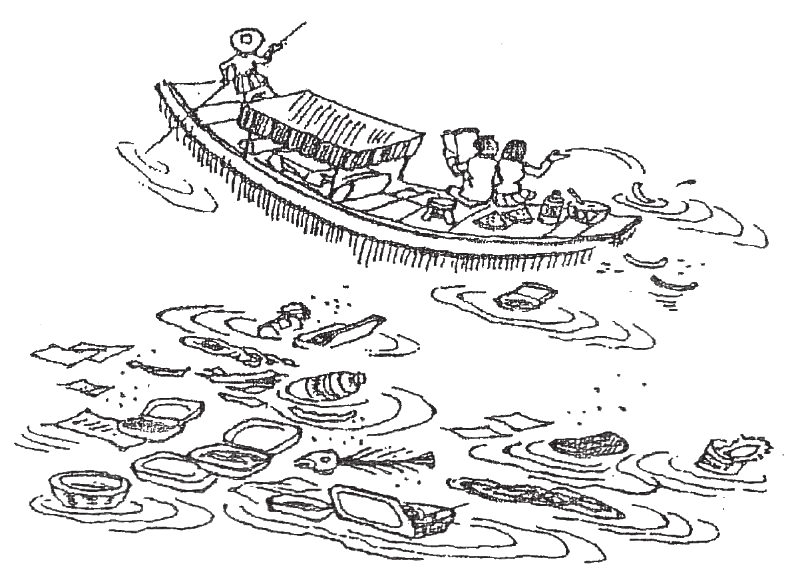
\includegraphics[width=0.54\linewidth]{picture/2011.png}
	\caption*{旅程之“余”}
\end{figure}

\checkpagenumber